
%(BEGIN_QUESTION)
% Copyright 2015, Tony R. Kuphaldt, released under the Creative Commons Attribution License (v 1.0)
% This means you may do almost anything with this work of mine, so long as you give me proper credit

\noindent
{\bf Programming Challenge -- model rocket launch timer with HMI screen} 

\vskip 10pt

Suppose we wish to automate a model rocket launchpad using a PLC to time the launch of the rocket.  When the ``Countdown'' pushbutton (momentary contact) is pressed, the PLC will begin a counting sequence to launch the rocket.  After 10 seconds, a discrete output point on the PLC will activate to power the rocket engine's igniter.

\vskip 10pt

Write a PLC program to perform this countdown function, and program an HMI to display the 10-second count from beginning to end in the form of a bargraph.

\vskip 20pt \vbox{\hrule \hbox{\strut \vrule{} {\bf Suggestions for Socratic discussion} \vrule} \hrule}

\begin{itemize}
\item{} How can you make this function latching, so that no one needs to hold the ``Countdown'' pushbutton the entire 10 seconds, but rather merely needs to press it once and release?
\end{itemize}

\vfil 

\underbar{file i02349}
\eject
%(END_QUESTION)





%(BEGIN_ANSWER)


%(END_ANSWER)





%(BEGIN_NOTES)

Here is one example of a workable solution for Allen-Bradley PLCs, where {\tt I:0/0} is the ``Launch'' pushbutton input, and a second timer ({\tt T4:1}) maintains power to the rocket ignitor ({\tt O:0/0}) for two seconds after the 10-second countdown completes:

$$\includegraphics[width=15.5cm]{i02349x01.eps}$$

If we don't mind holding the ``Launch'' pushbutton during the entire 10-second countdown, we may simplify the program to a simple {\tt TON} timer instruction driven by {\tt I:0/0}!




\vfil \eject

\noindent
{\bf Summary Quiz:}

(The recommended summary quiz is to have \underbar{each student} demonstrate their PLCs running this particular program)

%INDEX% PLC, programming challenge: model rocket launch timer with HMI screen

%(END_NOTES)


